\title{Milestone 3}
\author{Singularity Software}
\date{\today}

\documentclass[12pt]{article}
\usepackage[a4paper]{geometry}
\usepackage{makeidx}
\usepackage{lscape}
\usepackage{amsmath}
\usepackage{graphicx}
\usepackage[final]{pdfpages}

\geometry{top=1.0in, bottom=1.0in, left=1.0in, right=1.0in} % Sets the margins

\setlength{\parindent}{0pt} % Fixes the paragraph spacing problem

\renewcommand*\arraystretch{1.5}

\begin{document}

\begin{center}
	\LARGE{Milestone 3} \\
	\Large{\textit{Singularity Software}} \\
	\vspace{.05in}
	\normalsize{\today} \\
\end{center}

\section*{Sprint 2 Backlog}
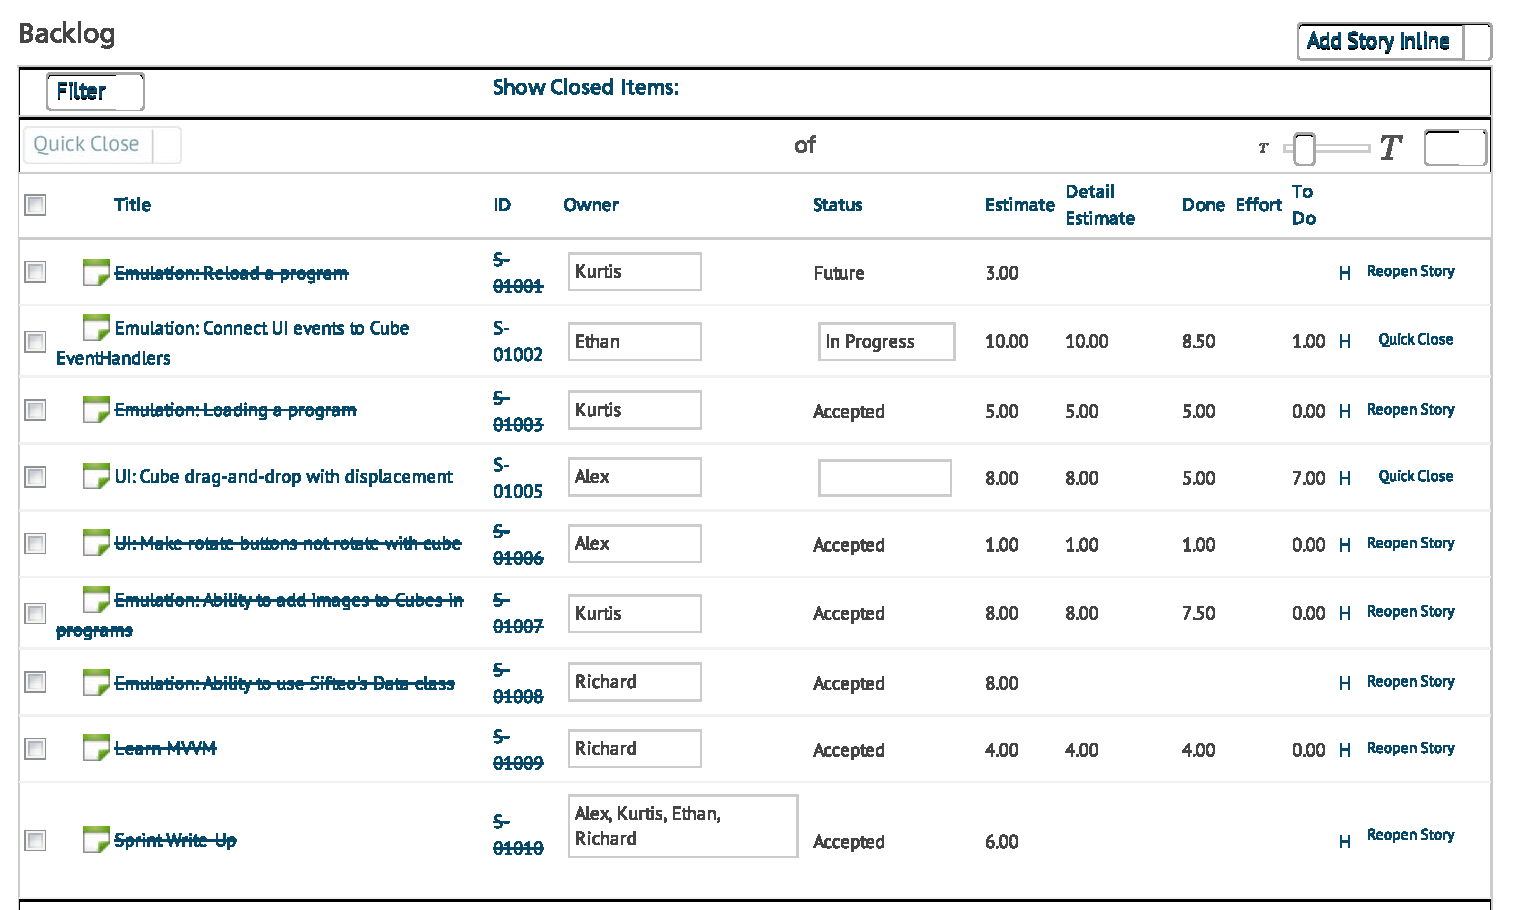
\includegraphics[scale=.63]{pdfs/MS2VersionOne/OldSprintBacklog_cropped.pdf}

\clearpage

\section*{Sprint 3 Backlog}
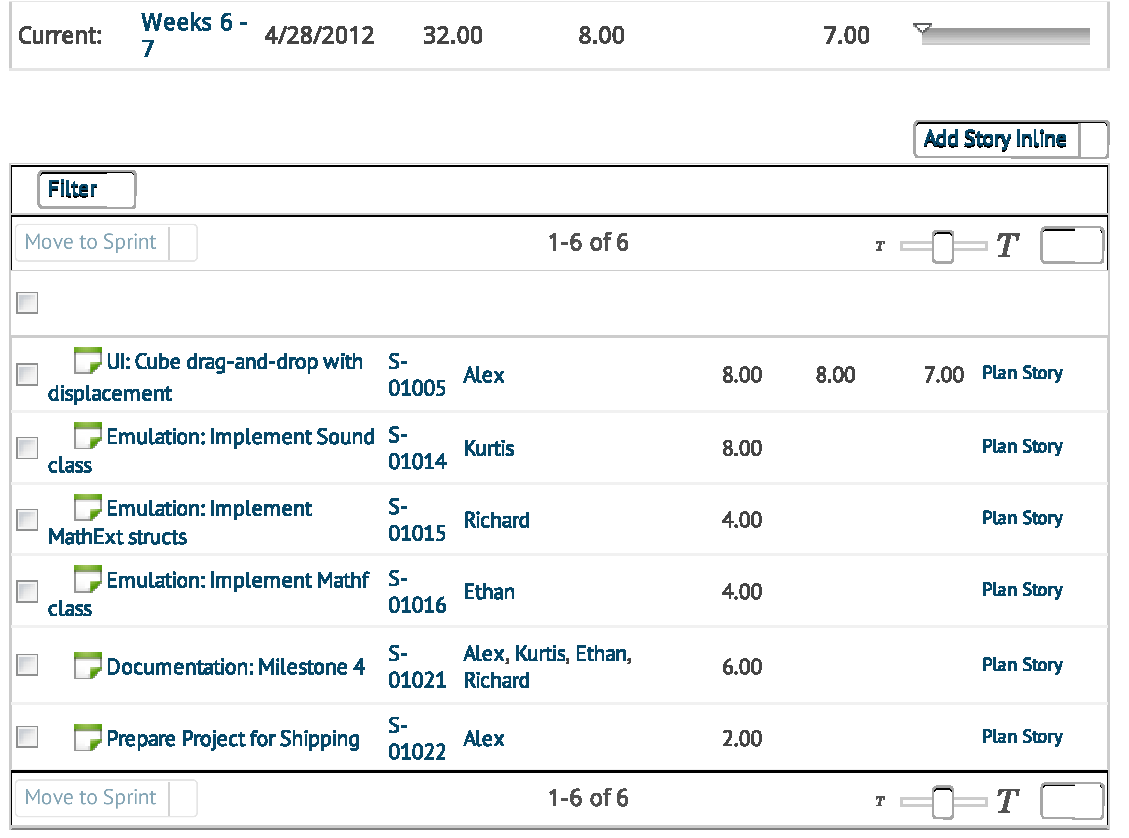
\includegraphics[scale=.85]{pdfs/MS3VersionOne/NewSprintBacklog_cropped.pdf}

\section*{Test-Driven Development}

\subsection*{Framework}
We used the Silverlight Unit Test Framework made available by Microsoft at \\ \underline{http://silverlight.codeplex.com/releases/view/78435}. We chose it because it ios designed by the same people who work on the Silverlight runtime and was therefore easy to integrate into our solution. This easy integration kept the amount of time required for TDD setup low.

\subsection*{Effects on Development}
We found that TDD didn't really slow down our development process significantly. Because we're still unfamiliar with many of the intricacies of the Sifteo API, there was and continues to be a lot of time spent simply understanding what each API class does before we start to implement it. In this regard, TDD was very helpful because it forced us to understand each class as we implemented the tests for it. This in turn tended to ensure that we understood each class in small increments instead of struggling to comprehend the entire class all at once.
\\\\
We found that TDD didn't really slow down our development process significantly. Because we're still unfamiliar with many of the intricacies of the Sifteo API, there was and continues to be a lot of time spent simply understanding what each API class does before we start to implement it. In this regard, TDD was very helpful because it forced us to understand each class as we implemented the tests for it. This in turn tended to ensure that we understood each class in small increments instead of struggling to comprehend the entire class all at once.
\\\\
TDD didn't really have an opportunity to improve our design decisions because most of the development we're doing at this point directly mirrors the Sifteo API structure. Mainly, the process helped us ensure more complete coverage of the API.

        
\end{document}
